\documentclass[12pt,a4paper,UTF8]{ctexart}
\usepackage{geometry}%用于设置上下左右页边距
	\geometry{left=2.5cm,right=2.5cm,top=3.2cm,bottom=2.8cm}
\usepackage{xeCJK,amsmath,paralist,enumerate,booktabs,multirow,graphicx,subfig,setspace,listings,lastpage,hyperref,amssymb,upgreek}
\usepackage{fancyhdr}
	\pagestyle{fancy}
	\rhead{实验 B13 利用超声光栅测量液体中的声速}
	\lhead{基础物理实验\uppercase\expandafter{\romannumeral2}实验报告}
	\cfoot{Page \thepage/\pageref{LastPage}}  %当前页\总页数
	\renewcommand{\headrulewidth}{0.4pt}
	\renewcommand{\theenumi}{(\arabic{enumi})}
	\setlength\headheight{15pt}

\begin{document}

\begin{center}
\LARGE\textbf{实验 B13 利用超声光栅测量液体中的声速}
\end{center}

%%信息
\begin{doublespacing}
	\centering
	\begin{tabular}{lr}
& \\
	{\CJKfontspec{方正楷体简体} 学院:中山医学院} & {\CJKfontspec{方正楷体简体} 年级、专业:2020级临床医学(长学制)} \\
	{\CJKfontspec{方正楷体简体} 实验人姓名、学号:莫润冰~20980131} & {\CJKfontspec{方正楷体简体}合作者姓名:张誉之~20980100}\\
	{\CJKfontspec{方正楷体简体} 实验时间:2021年9月30日~星期四~上午} & {\CJKfontspec{方正楷体简体} 室温:27$^{\circ}$C~ 相对湿度:56\%}
	\end{tabular}
\end{doublespacing}


振动频率超过20kHz的机械波称为超声波,因为具有方向性好、穿透能力强、易于聚焦、在水中传播距离远等特点,因此在测距、测速、清洗、焊接、消毒、声纳定位等医学、
军事和工农业领域得到广泛应用。

\subsection*{【实验目的】}
	\begin{enumerate}
		\item 了解超声波的基本性质并掌握超声光栅的工作原理
		\item 学会利用超声光栅测量液体中的声速
	\end{enumerate}

\subsection*{【实验仪器】}
\begin{table}[htbp]
	\centering
    \begin{tabular}{cccp{20em}}
	\toprule
	编号    & 仪器用具名称 & 数量    & 主要参数(型号,测量范围,测量精度等) \\
	\midrule
	1     & 超声光栅池 & 1     & \\
	2     &超声光栅声速仪 & 1 & KF-WSG \\
	3     & 分光计 & 1 & KF-JJY1\\
	4     & 低压钠灯 & 1 & KF-GP20Na\\
	5     & 测微目镜(或电子目镜)& 1 & JX8\\ 
	\bottomrule
	\end{tabular}%
	\label{tab:device}%
\end{table}%

\subsection*{【实验原理】}
\subsubsection*{1.超声光栅的形成}

\begin{figure}[htbp]
	\centering
	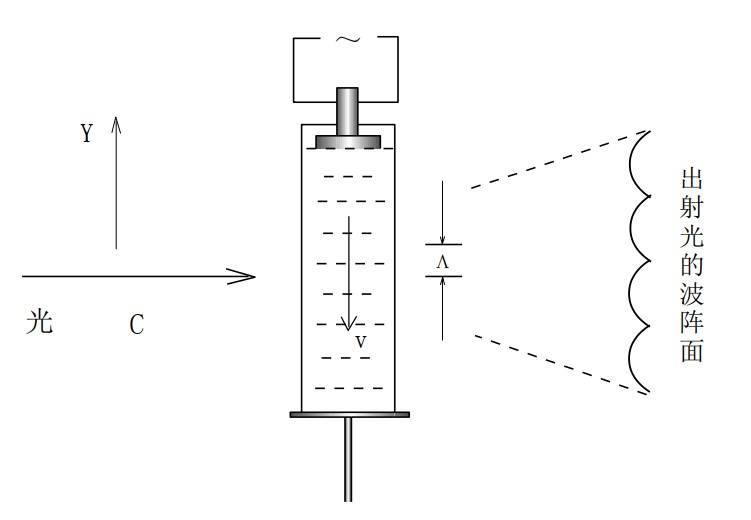
\includegraphics[width=0.6\textwidth]{img//1.jpg}
	\caption{超声光栅的形成示意图}
\end{figure}

具有弹性纵向的平面超声波,在液体介质中传播时,其声压使液体分子产生疏密交叠的变化,促使液体的折射率也相应的作周期性变化。
当光沿垂直方向透射过超声场后,会产生折射和衍射。
这一作用,类似光栅,所以称为超声光栅。

\subsubsection*{2.超声波的速度与介质的性质}
超声在介质中传播的性质,一般用声速和衰减系数两个基本量来表述。超声波速度不仅与声压(p)、密度($\rho$ )、折射率(P、N)有关,而且还受其它物理性质影响。
在正弦变化的声场中,超声波运动的速度、声压以及介质的密度和折射率n的变化规律可以用波动方程表示。
超声场中折射率周期性变化的的表达式可写为:
\begin{equation}
	n(y,t)=n_0+\varDelta n cos(\omega t-ky)
\end{equation}

\subsubsection*{3.超声的驻波和行波}
正弦超声平面波由垂直于超声样品池侧面的压电陶瓷片射入液体中,如图1所示,则声场中的压力波会被侧面反射,形成与入射波同频率的一列反射波,这两列波的压强可以
分别表示为:

\begin{equation}
	\begin{cases}
		&P_i=P_{iA}e^{i(\omega t-ky)} \\
		&P_r=P_{rA}e^{i(\omega t+ky)}\\
	\end{cases}
\end{equation}

两列同效率的波反向传播时,依叠加原理,合成声场的声压为$P=P_i+P_r$,即

\begin{equation}
	P=2P_icos(kye^{i\omega t})+(P_{iA}-P_{rA})e^{i(\omega t-ky)}
\end{equation}

由上式可见,合成声场由两部分组成,第一项代表驻波场,第二项表示在Y方向进行的平面波场,其振幅为原先两列波振幅之差。
若实验中弹性的平面波得到完全反射,则式(3)y右边第二项可以略去。
合成的超声场就是一个纯粹的驻波场。介质密度分布和折射率的分布也与驻波场的变化相一致。
声压形成的光密处为波节,光疏处为波腹。如图2(a)所示。
从密度或折射率变化的相对位置看,如图(2b)在(t+T)/2时的波形相对于t时刻的波形来说,好像光栅相对向右移动了半个波长。
而在任何时刻相距为λ的两点处,液体的密度是相同的。
由于光向折射率大的方面弯曲,所以波节处交迭地每隔半个周期呈现一次汇聚强光。
这种周期性的变化人眼看不出来,实验观察到的超声场的图像,是相对的长时间的平均效应。
图3就是在声压作用下,超声场中介质疏密的瞬时分布。
行波的疏密波会向前传播。

\begin{figure}[htbp]
	\centering
	\subfloat[超声驻波的运动]{\label{fig:nogamma4}
	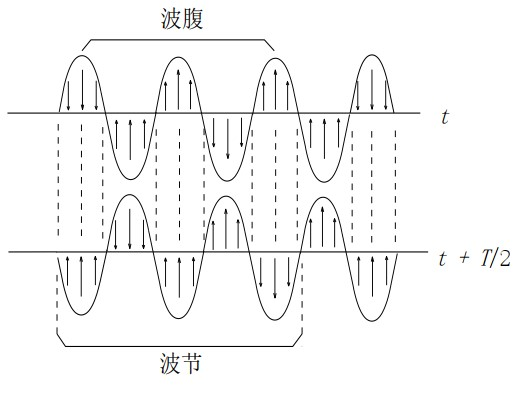
\includegraphics[width=0.4\textwidth]{img/2a.jpg}%调节这里的图片宽度
	}%
	\subfloat[超声驻波速度和声压的分布]{\label{fig:withgamma4}
	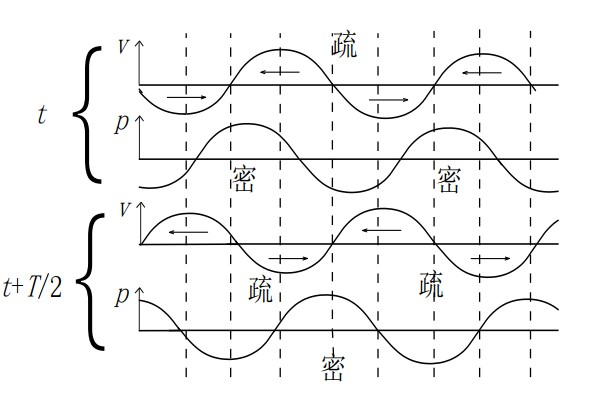
\includegraphics[width=0.4\textwidth]{img/2b.jpg}%调节这里的图片宽度
	}%
	\caption{}
	\label{fig:tcvi}
\end{figure}

\begin{figure}[htbp]
	\centering
	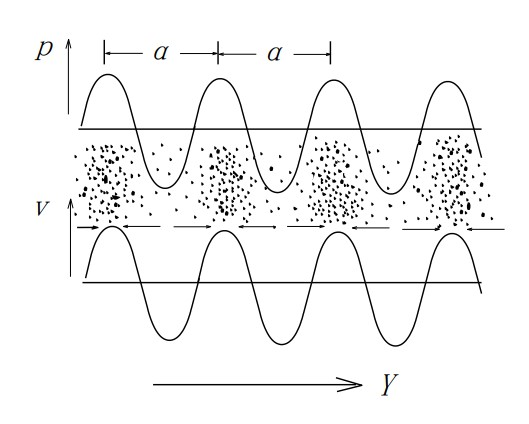
\includegraphics{img//3.jpg}
	\caption{}
\end{figure}

\subsubsection*{4.超声衍射的观测}
因光速远大于声速,即c≫u,光线很快的通过了超声场,而折射率不同层次所形成的“超声光栅”可以认为是不动的,即把折射率的空间固定的看成:
\begin{equation}
	N=N_0+\varDelta N cos(ky)
\end{equation}
这样所形成的超声光栅对光的衍射可表示为:
\begin{equation}
	\varLambda sin \theta_K = \pm K\lambda
\end{equation}
式(5)中$\varLambda $和$\lambda$分别为超声波和光波的波长,$\theta_K $为K级衍射角。
由该式可知,如果测出$\theta_K$,且$\lambda$已知,则可测出超声波的波长$\varLambda$ ,若知道超声波的频率f,则可求出超声波在该液体中的传播速度:
\begin{equation}
	u=\varLambda f
\end{equation}
这是测量超声波传播速度的有效方法之一。

\subsubsection*{5.超声场的观测}
采用图4(a)所示的光路,将超声光栅液体池AB放在分光计的载物台上,其中B为超声源。则可在望远镜中观察到如图4(b)所示的系列平行条纹。
利用分光计可以测量出每根条纹的衍射角,进而测出超声波的波长$\varLambda $,并根据超声波的频率f,利用式(6)计算出超声波在液体中传播的速度。

\begin{figure}[htbp]
	\centering
	\subfloat[超声光栅实验光路图]{\label{fig:nogamma4}
	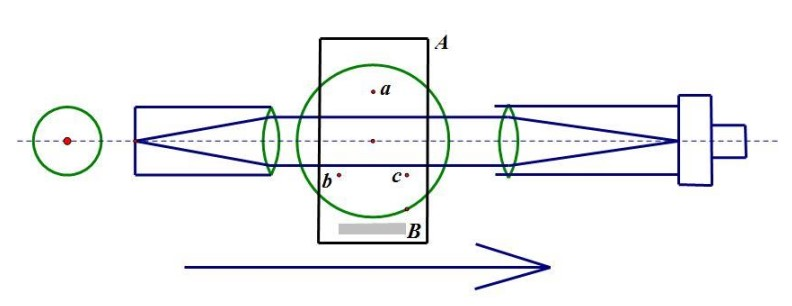
\includegraphics[width=0.7\textwidth]{img/4.jpg}%调节这里的图片宽度
	}%
	\subfloat[超声光栅成像]{\label{fig:withgamma4}
	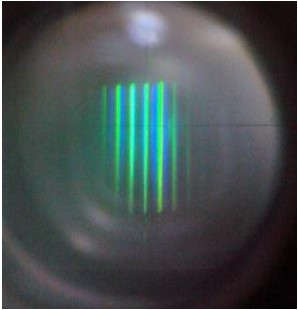
\includegraphics[width=0.3\textwidth]{img/5.jpg}%调节这里的图片宽度
	}%
	\caption{}
	\label{fig:tcvi}
\end{figure}

为提高测量精度,可将望远镜目镜换成测微目镜进行观察。
条纹像落在测微目镜的焦平面上,条纹清晰。用测微目镜测出条纹间距x,可将条纹的衍射角表示为

\begin{equation}
	tan \theta_K\approx sin\theta_K=\frac{x}{F}
\end{equation}
其中F为测微目镜的焦距。根据式(5)和式(7)可得
\begin{equation}
	\frac{K\lambda}{\varLambda }=\frac{x}{F}
\end{equation}
则
\begin{equation}
	\frac{x}{fF}=\frac{\lambda}{f\varLambda}=\frac{\lambda}{u}
\end{equation}
其中u是要测的声速,f为超声波的频率,则被测液体中的声速可表示为
\begin{equation}
	u=\frac{\lambda F f}{x}
\end{equation}

\subsection*{【安全注意事项】}
    \begin{enumerate}
		\item 实验结束,超声池中的水应尽快清理,不应长时间浸泡在液体槽内。
		\item 超声仪的频率易受外界环境的影响,只要外界变化使其导线电容分布发生变化,就有可能会对输出频率产生影响,应尽量避免震动及触碰导线。
		\item 若该实验原配的超声信号发生器工作不稳定,可采用函数信号发生器替代,但采用原厂设备可观察到3级衍射谱,采用替代设备只能观察到2级衍射谱。同时函数信号发生器的输出信号峰峰值不要超过18V。
	\end{enumerate}

\subsection*{【实验装置】}
实验装置如图5所示。若不采用测微目镜,只是使用分光计测量超声光栅的衍射角,则可不安装测微目镜(8),采用望远镜目镜和显示器代替。
\begin{figure}[htbp]
	\centering
	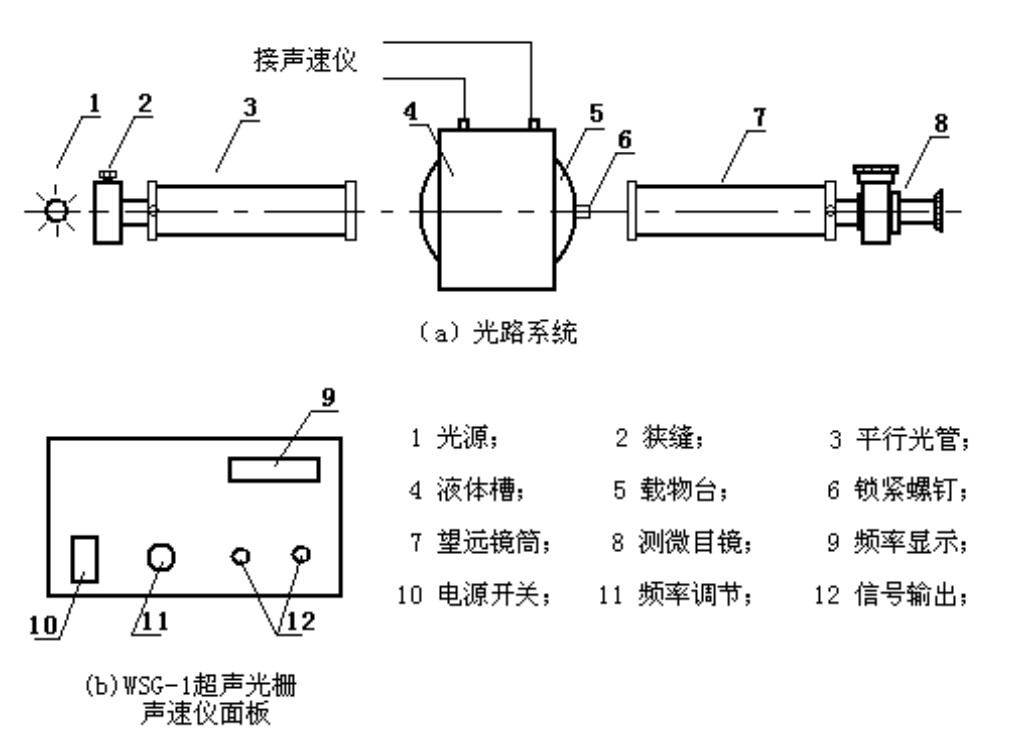
\includegraphics[width=0.8\textwidth]{img//6.jpg}
	\caption{超声光栅实验装置图}
\end{figure}


\subsection*{【实验内容及步骤】}

\subsubsection*{1.实验装置调节}
    \begin{enumerate}
		\item 调节分光计到正常测量状态,平行光管与望远镜准直同轴。
		\item 在超声光栅盒中加入适量的水,并固定在分光计载物台上。转动游标盘使光栅盒正面玻璃反射的绿色十字像的垂直线和水平线与十字叉丝的垂直线和水平线重合。并连
		接超声盒电路。
		\item 打开光源,在望远镜中可看到一条竖直亮条纹。微调望远镜和狭缝宽度使条纹清晰,并使条纹与望远镜垂直叉丝重合。记录角度$\theta_0$.
		\item 打开超声源开关,微调超声波频率,使视野中出现尽可能多的衍射条纹且条纹清晰。
	\end{enumerate}

\subsubsection*{2.采用衍射角法测量声速}

直接采用分光计的望远镜目镜,测量不同条纹的衍射角,根据式(5)和式(6)计算液体中超声波的波长$\varLambda$ 计算液体中声速u.
\subsubsection*{3.采用测微目镜测量声速}

采用测微目镜替换望远镜目镜。在观察到清晰条纹后,转动测微目镜上的鼓轮,测量每条条纹的位置,用逐差法求出条纹间距x,利用式(10)计算液体中声速u.
请自列表格记录数据和计算,并分析结果的不确定度。

\subsubsection*{4.选做实验}
    \begin{enumerate}
		\item 选做内容1:对比正弦信号和方波信号驱动下超声光栅衍射条纹的异同。
		\item 选做内容2:改变液体温度,测不同温度下液体中的声速,寻求变化规律。		
	\end{enumerate}

\subsection*{【实验数据处理】}

\subsubsection*{1. 采用衍射角法测量纯水声速}
		\paragraph{实验参数} 钠黄光波长$\lambda = 589.3 nm$,超声频率$f = 11.109 MHz$
		\paragraph{实验数据}~
		\newline
		\indent
		利用分光计望远镜目镜,测量超声光栅不同级次条纹的衍射角,原始数据如表\ref{tab:1}。

\begin{table}[htbp]
	\centering
	\caption{实验数据记录}
	\begin{tabular}{cccccc}
	\toprule
	条纹级数k    & -2 & -1  & 0 & 1 & 2 \\
	\midrule
	游标1     & 44$^{\circ}$16' & 44$^{\circ}$0' & 43$^{\circ}$45'&  43$^{\circ}$30'   & 43$^{\circ}$15'\\
	游标2     & 224$^{\circ}$13' & 223$^{\circ}$58' & 223$^{\circ}$43' & 223$^{\circ}$28' & 223$^{\circ}$14' \\
	均值      & 134$^{\circ}$14'30" & 133$^{\circ}$59' & 133$^{\circ}$44' & 133$^{\circ}$29' & 133$^{\circ}$14'30"\\
	衍射角$\theta_k$    & -30'30" & -15' & 0 & 15' & 29'30" \\
	$sin\theta_k$    &   -8.87$\times 10^{-3}$ & -4.36$\times 10^{-3}$ & 0 &4.36$\times 10^{-3}$ & 8.58$\times 10^{-3}$ \\
	\bottomrule
	\end{tabular}%
	\label{tab:1}%
\end{table}%


		计算k级条纹角度值与零级条纹角度值之差,得到各级条纹角位置,并计算正弦值。
		
		\paragraph{拟合$k-sin\theta_k$曲线计算声速值}~
		\newline
		\indent
		拟合$k-sin\theta_k$曲线,结果如图\ref{fig:1}。直线斜率为229.22。
		\begin{figure}[htbp]
			\centering
			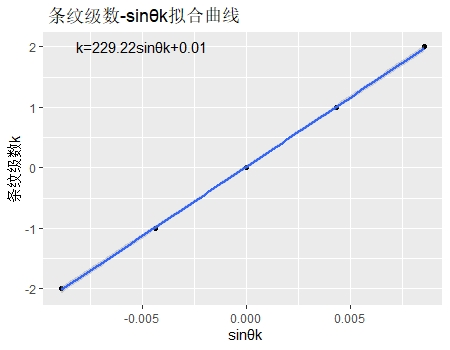
\includegraphics[width=0.7\textwidth]{img//curve1.jpeg}
			\caption{拟合$k-sin\theta_k$曲线}
			\label{fig:1}
		\end{figure}
		
		由式5和式6得声速计算公式
		\begin{equation}\label{eq:5}
			u = f\lambda\frac{k}{sin(\theta_k)}
		\end{equation}
		
		代入直线斜率和实验参数,计算得
		$$
		u = 1500.60 m/s
		$$


\subsubsection*{2. 采用测微目镜测量声速}
		\paragraph{实验参数} 钠黄光波长$\lambda = 589.3 nm$,超声频率$f = 11.042 MHz$,测微目镜焦距$F = 170mm$
		\paragraph{实验数据}~
		\newline
		\indent
		利用测微目镜,测量超声光栅不同级次条纹的位置,原始数据如表\ref{tab:2}。$k$为衍射级次,$x$为条纹位置

\begin{table}[htbp]
	\centering
	\caption{实验数据记录}
	\begin{tabular}[width=textwidth]{cccccc}
	\toprule
	条纹级数k    & -2 & -1  & 0 & 1 & 2 \\
	\midrule
	条纹位置/mm    & 3.398 & 4.107 & 4.896 & 5.650 & 6.369 \\
	条纹角位置x/mm   & -1.498 & -0.709 & 0 & 0.754 & 1.473 \\
	\bottomrule
	\end{tabular}
	\label{tab:2}
\end{table}

\paragraph{拟合$k-x$曲线计算声速值}~
		\newline
		\indent
		拟合$k-x$曲线,结果如图\ref{fig:2}。直线斜率为1.350。
		\begin{figure}[htbp]
			\centering
			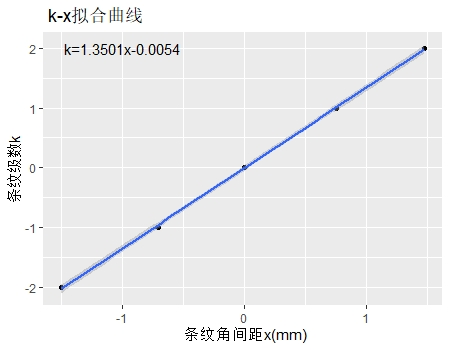
\includegraphics[width=0.7\textwidth]{img/curve2.jpeg}
			\caption{拟合$k-x$曲线}
			\label{fig:2}
		\end{figure}
		
		由声速计算公式(10),式中$x$为条纹角间距,即为上述拟合直线斜率的倒数。代入直线斜率和实验参数,计算得
		$$
		u = 1493.37 m/s
		$$

\subsection*{【实验结果分析】}
查得实验条件下声速理论值$u = 1502.04 m/s$。

衍射角法测量值为$u = 1500.60 m/s$,相对误差为$0.0096\%$

测微目镜法测量值为$u = 1493.37 m/s$,相对误差为$0.058\%$

可见衍射角法测量声速能获得更高的准确度。
这是因为实验时所用测微目镜与分光计不适配,在衔接处固定不紧,轻微扰动就能造成较大误差。



\subsection*{【思考题】}
\subsubsection*{(1)由驻波理论知道,相邻波腹间的距离和相邻波节间的距离都等于半波长,为什么超声光栅的光栅常数等于超声波的波长呢?}
答:超声波在液体中以纵波的形式传播,在波前进的道路上,液体被周期性的压缩与膨胀,其密度产生变化,形成所谓的疏密波。
在一定条件下,前进波与反射波叠加形成驻波。
其中振幅最大的位置称为主播的波腹,振幅为0的位置称为驻波的波节。
对任意波节而言,它两边的质点在某一时刻都涌向节点,使波节附近成为质点密集区,半周期后,节点周围的质点又向左右散开,使波节附近成为质点稀疏区。
在同一时刻,相邻两个波节附近质点分布情况正好相反。
而超声光栅的光栅常数等于两个密集区或者两个稀疏区之间的距离,这正好是相邻波腹或者波节之间距离的二倍,因此光栅常数正好等于超声波的波长。

\subsubsection*{(2)比较超声光栅与平面光栅的异同。}
超声光栅:由超声波在液体中产生的光栅作用称作超声光栅。超声波作为一种纵波在液体中传播时,其声压使液体分子产生周期性的变化,促使液体的折射率也相应地作周期性的变化,形成疏密波。此时,如有平行单色光垂直于超声波传播方向通过这疏密相同的液体时,就会被衍射,这一作用,类似光栅,所以称为超声衍射。
平面衍射光栅:普通的光线衍射光栅。
相同:当有光透过时,两种光栅都能使光发生衍射现象并得到衍射图样。超声光栅的衍射光强分布与平面衍射光栅几乎无区别。
不同:超声光栅是一种可擦除的实时光栅,它的光栅常数可以通过超声波的频率和振幅来控制。因此,相比平面衍射光栅有更大的可调节性。

\subsubsection*{(3)有的教材中,超声光栅实验的超声波频率为200kHz,请问此时能用光栅的原理解释实验结果吗?为什么?}
不能。超声波的频率增大会使形成的超声光栅的光栅常数增大,由公式$dsin\theta=n\lambda$知,d减小$\lambda$不变则$sin\theta$ 增大,条纹间距增大。光栅的原理是当光栅常数较小时成立的,当频率过高时,衍射条纹间距过宽,$sin\theta$与$\theta$的近似性不再成立,因此这时光栅的原理不再适用于解释实验现象。
\end{document}
